%\documentclass[11pt,twoside,a4paper]{article}
\documentclass[11pt,a4paper]{article}
\usepackage[italian]{babel}
\usepackage{listings}
\usepackage{color}
\usepackage{mathtools}
\usepackage{biblatex}
%useful colors
\definecolor{mygreen}{rgb}{0,0.6,0}
\definecolor{mygray}{rgb}{0.5,0.5,0.5}
\definecolor{mymauve}{rgb}{0.58,0,0.82}
\definecolor{gray}{rgb}{0.4,0.4,0.4}
\definecolor{darkblue}{rgb}{0.0,0.0,0.6}
\definecolor{cyan}{rgb}{0.0,0.6,0.6}
%defining styles for listings
%java listings
\lstdefinestyle{octave}{
	basicstyle=\footnotesize,
	breakatwhitespace=false,
	breaklines=true,
	captionpos=b,
	commentstyle=\color{mygreen},
	frame=single,
	keywordstyle=\color{blue},
	language=octave,
	numbers=left,
	numbersep=5pt,
	numberstyle=\tiny\color{mygray},
	rulecolor=\color{black},
	showstringspaces=false,
	stepnumber=1,
	stringstyle=\color{mymauve},
	tabsize=2,
	title=\lstname
}
\begin{document}
\title{Classification on Pedobarography images}
\author{Luigi Lomasto, Marco Mecchia} 
\maketitle
\section{Introduzione al problema}
IL termine Pedobarography deriva dal latino \emph{pedes}, piede, e dal greco \emph{baros}, peso o pressione, e si riferisce allo studio dei campi di pressione della superficie plantare del piede su una superficie di supporto. La Pedobarography \'e spesso usata per l'analisi biomeccanica del movimento animale e per l'analisi della postura. In questo lavoro, il nostro obiettivo \'e quello di addestrare un sistema di Machine Learning in grado di classificare le immagini derivate dall'analisi statica, tramite Pattern Recognition Statistico.
Il resto del lavoro \'e organizzato come segue: nella sezione \ref{sec:dataset} viene descritto il dataset utilizzato nel lavoro, e il lavoro di preprocessing effettuato su di esso. Nella sezione \ref{sec:features} vengono descritte le feature scelte per addestrare il classificatore, e la loro convalida tramite metodi noti in letteratura. Nella sezione \ref{sec:classification} vengono descritti i classificatori utilizzati. Nella sezione \ref{sec:results} vengono illustrati i risultati, ed infine nella sezione \ref{sec:conclusions} vengono tratte le considirezioni su quanto fatto, ed analizzati alcuni possibili sviluppi futuri.

\section{Dataset}
\label{sec:dataset}
Il dataset utilizzato consiste in 100 immagini derivate dall'analisi statica di 100 pazienti diversi, ed \'e stato fornito dal dott. NOME DOTTORE in forma anonima. Un esempio di immagine \'e fornito in figura \ref{fig:immagineEsempio}. 
\begin{figure}
\centering
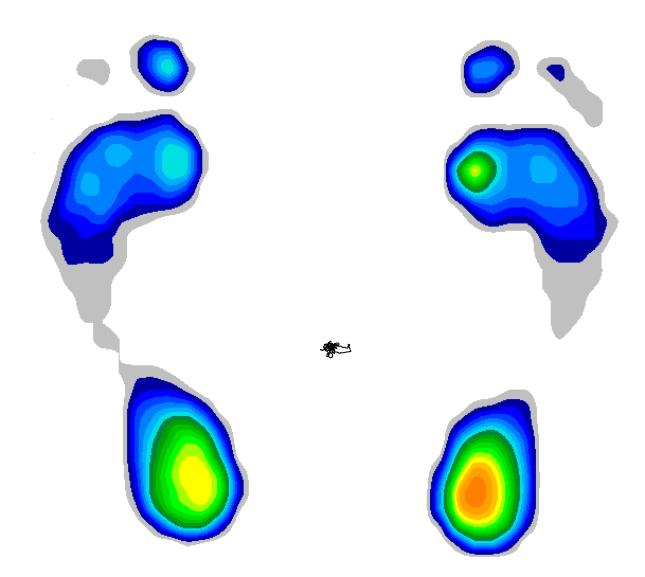
\includegraphics[width=300px, keepaspectratio]{esempio.png}
\label{fig:immagineEsempio}
\caption{Un immagine del dataset}
\end{figure}
Per ogni immagine ci \'e stata fornita anche la patologia di cui era affetto il piede del paziente, esse sono:
\begin{description}
\item[Piede Valgo] Sinistro, Destro, o Bilaterale.
\item[Piede Cavo] Sinistro, Destro, o Bilaterale.
\item[Piede Piatto] Sinistro, Destro, o Bilaterale.
\item[Piede Normale] Sinistro, Destro, o Bilaterale.
\end{description}

Tutte queste patologie non sono necessariamente esclusive: in particolare, un piede valgo pu\'o anche essere piatto o cavo. Per questo motivo, e per non gestire troppe classi di output, la classificazione \'e stata organizzata in maniera gerarchica, come si pu\'o vedere in figura \ref{fig:classificazioneGerarchica}.

FIGURA/DIAGRAMMA DI FLUSSO

Ogni immagine viene suddivisa in piede sinistro e piede destro. Sul piede singolo prima viene effettuata la classificazione cavo vs piatto, in quanto le classi sono mutualmente esclusive, dopodich\'e viene effettuata la classificazione valgo vs non valgo. Le informazioni sui piedi vengono combinate alla fine per stabilire se la patologia \'e bilaterale o meno.

\subsection{Preprocessing}

Prima di estrarre le features dalle immagini, \'e stato necessario un lavoro di preprocessing su tutto il dataset. Come si pu\'o vedere nella figura \ref{fig:esempio}, in ogni immagine al centro c'\'e il tracciato del baricentro durante l'analisi statica. Tale tracciato viene utilizzato dal medico per questioni relative alla postura ed al bilanciamento del corpo, quindi non \'e utile al fine della nostra classificazione. Per questo motivo, il primo passo \'e stato eliminare tale tracciato da ogni immagine. Abbiamo utilizzato una semplice funzione in matlab/octave che funziona nella maggioranza dei casi. Per i casi al limite, cio\'e quelli in cui si rischiava di cancellare anche parte di un piede, la rimozione \'e stata fatta manualmente.

\lstinputlisting[style=octave, caption=Image Cleaner Function]{../FeatureExtraction/clearImage.m}

\section{Feature Extraction}
\label{sec:implementation}

\end{document}
